\documentclass{article}

% For figures
\usepackage{graphicx} % more modern
\usepackage{subfigure} 

% For citations
% \usepackage{natbib}

% For algorithms
\usepackage{algorithm}
\usepackage{algorithmic}

\usepackage{hyperref}

% Packages hyperref and algorithmic misbehave sometimes.  We can fix
% this with the following command.
\newcommand{\theHalgorithm}{\arabic{algorithm}}

% \usepackage{sty/icml2013} 
% Employ this version of the ``usepackage'' statement after the paper has
% been accepted, when creating the final version.  This will set the
% note in the first column to ``Proceedings of the...''
\usepackage[accepted]{sty/icml2013}


% The \icmltitle you define below is probably too long as a header.
% Therefore, a short form for the running title is supplied here:
\icmltitlerunning{Clustering and Topic Discovery in Gene Expression Data}

\begin{document} 

\twocolumn[
\icmltitle{Bayesian Clustering and Topic Discovery: \\ 
           Adventures with Gene Expression Data}

% It is OKAY to include author information, even for blind
% submissions: the style file will automatically remove it for you
% unless you've provided the [accepted] option to the icml2013
% package.
\icmlauthor{Karren Dai Yang, Skanda Koppula}{\{karren, skoppula\}@mit.edu}
\icmladdress{Massachusetts Institute of Technology,
            Cambridge, MA 02139 USA}

\icmlkeywords{topic models, bayesian clustering, gene expression, gene modules}

\vskip 0.3in
]

\section{Introduction}
\label{intro}
Tumors cell lines are composed of different sub-populations of cells which often exhibit shared patterns of gene expression. Biologists are interested in two key questions: given gene expressions values, (1) can we identify cell clusterings, and (2) can we identify clusters of biologically-related genes? Our goal with this project was to answer both these two questions using Bayesian methods.

In brief, we explored the use of three Bayesian clustering methods (a vanilla mixture, integrated topic-mixture, and non-parametric models) to address the first question, and two topic models (vanilla and a dynamic-topic LDA) to address the second. 

\subsection{Description of Data}
Using a contemporary gene sequencing machine, we obtained samples of single-cell RNA-sequencing data (scRNA-seq) taken from tumors in mice. Our data consisted of the expression values of 22,712 genes for each of 4645 cells. In total, the dataset amounted to 0.86 GB, presenting significant computational challenges when attempting posterior estimation. Apart from a few computational tricks (online inference, multi-core parallelization), for most methods, we pruned non-informative genes from the dataset, ranking based on the deviation in value across cells \footnote{We recognize that this can bias towards noisy genes. We favor this method because it is simple and easy to implement, and a practice used in literature \cite{pruning}}. The Seurat biological toolkit in R was also used for the purpose of low-variance feature selection \cite{seurat}. We eschewed dimensionality reduction techniques such as PCA because of loss of its direct feature interpretability. Prior researchers have labeled the cells in our dataset; there are a total of 9 cell categories. The complete dataset, as well our preprocessed and pruned versions, are openly available \cite{dataset}.

\subsection{Prior work}
Prior research has explored the use of various computational techniques to analyze gene expression data. Most commonly, Spearman and Pearson correlation metrics are frequently used infer sets of genes that cluster together \cite{profiling, nature}. Other techniques, including PCA followed by linear regression, has been used for expression-based cell clustering \cite{transcriptomics}. Yu et al. propose an unsupervised classifier ensemble as another approach to cell clustering \cite{consensus}. 

More Bayesian approaches have also been tried in prior work from the Pe'er lab. \cite{bayesge2} uses a Heirarchical Dirichlet Mixture Model to learn cell clusterings. \cite{bayesge1} builds on this to jointly learn optimal normalization pre-processing of the data. Bayesian networks have also been used in an attempt to learn gene dependencies from expression data \cite{bayesge3}. Our work uses different models to explore gene expression data, but where appropriate (e.g. in mixture models in Section~\ref{mmsec}), we compare results.

\subsection{Structure of Report}
We first discuss our experiments using Bayesian topic models to discover related sets of genes in a 'topic': LDA in Section~\ref{ldasec} and Dynamic Time Models in Section~\ref{dtmsec}. Then, we discuss our experiments in clustering: Dirichlet Mixtures in Section~\ref{mmsec}, Integrated Topic-Clustering in Section~\ref{intsec}, and non-parametric models in Section~\ref{nonparametricsec}. We conclude our paper with our observations from across all our studies. 

For the purpose of reproducibility, all code can be found at \url{https://github.com/skoppula/882}.

\section{Latent Dirichlet Allocation} 
\label{ldasec}
\subsection{Model Description} 
In the generative process for LDA, the topic assigned to each word is a drawn from the document's topic distribution. The identity of the word is drawn from topic's word distribution. Assuming the reader is familiar with LDA, we relegate further details and formalization of the model to \cite{LDA}.

In the context of analyzing gene expression data, we are interested in discovering 'topics' that comprise of a set of top-$N$ genes within the topic distribution that are biologically related. For example, together the genes may direct a specific chemical function in a cell. Biologists denote such sets of genes as 'gene modules' which can be cross-referenced with existing gene module databases.

\subsection{Implementation} 
A first attempt using the built-in Python \texttt{lda} package resulting in early memory overflows during what we suspect was pre-allocation of per-document variables. The source code was not available, so we had few clues.

We switched to two open-source implementations: an online mean-field variational Bayes for posterior estimation \cite{ovb}, and a broken \texttt{C++} Gibbs sampler for LDA \cite{plda}. 

\nocite{online}

We fixed portions of the sampler to compile properly and extended the sampler to run in across four cores. Details of our sampling procedure can be found in Appendix~\ref{ldaappendix}. We compared these two posterior estimation approaches using our entire dataset, using a 10\% held-out testing partition. We experimented using $k=5, 10, 25, 50$ topics. We did not require dataset pruning after these optimizations.

\subsection{Experiments} 
- posterior predictive checks
- no intrusion testing meaningful
- hypergeometric tests
- likelihood
- performance metrics

We did gene set enrichment analysis using the minimum hypergeometric test \cite{hg} to compare our topics, which are ranked lists of genes, with existing collections of genes catalogued in the comprehensive gene module database, \texttt{MSigDB} \cite{msigdb}. Figure \ref{fig:pathways} in the Appendix shows topic-to-\texttt{MSigDB} module matches for which the $p$-value of the match is at least less than 0.3. Models with more topics tended to have more matches with higher significance. These results suggest that we need to train the model with more topics. We note that the $p$-values do \textit{not} factor for multiple hypothesis corrections, so at the moment we are only using them as relative measures of model quality.

3. More details about biological significance: Good question about \# of topics affecting the results for the hypergeometric test for biological relevance/correlation with existing biologically annotated. This is something I'm not too sure about, and why we experience the results we do. That said, \# topics is something that we were experimented with, but soon realized we didn't consider a broad enough range, after seeing the results from our non-parametric model afterward. More
investigation and thought will need to go into this for the final report.

Figure \ref{fig:time} shows the time to complete each estimation method. As expected, Gibbs scales poorly with the parameter dimensionality and is strictly worse than online variational Bayes across all studied topic counts. We also calculated perplexity and log-likelihood for the OVB parameters, and very surprisingly, we found that log-likelihood decreased as number of topics increased on a held-out test set (Figure \ref{fig:ll}). We are currently trying to understand whether this is because of programming error.


\begin{figure}[h]
\vskip 0.2in
\begin{center}
\centerline{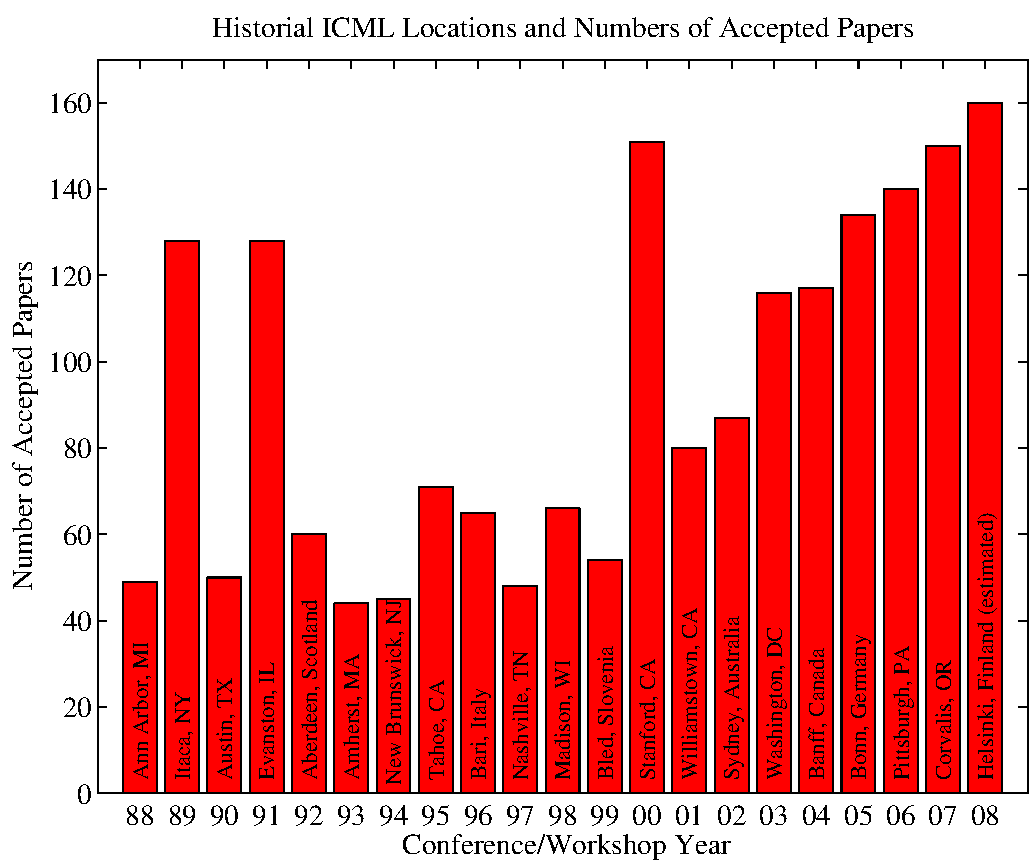
\includegraphics[width=\columnwidth]{figs/examplegraph}}
\caption{This is a demo figure.}
\label{alabel}
\end{center}
\vskip -0.2in
\end{figure} 


\section{Dirichlet Mixture Model} 
\label{mmsec}
\subsection{Model Description} 
    Algorithm~\ref{alg:example} describes the generative process for the mixture odel.

    \begin{algorithm}[tb]
       \caption{Mixture Model}
       \label{alg:example}
    \begin{algorithmic}
       \STATE {\bfseries Input:} data $x_i$, size $m$
       \REPEAT
       \STATE Initialize $noChange = true$.
       \FOR{$i=1$ {\bfseries to} $m-1$}
       \IF{$x_i > x_{i+1}$} 
       \STATE Swap $x_i$ and $x_{i+1}$
       \STATE $noChange = false$
       \ENDIF
       \ENDFOR
       \UNTIL{$noChange$ is $true$}
    \end{algorithmic}
    \end{algorithm}
\subsection{Implementation} 
\subsection{Experiments}  
- comparison with pe'er paper


\section{Dynamic Time Model} 
\label{dtmsec}
\subsection{Model Description} 
\subsection{Implementation} 
\subsection{Experiments} 


\section{Integrated Topic-Clustering Model} 
\label{intsec}
\subsection{Model Description} 
\subsection{Implementation} 
\subsection{Experiments} 



\section{Non-parametric Models: IBP and HDP} 
\label{nonparametricsec}
\subsection{Model Description} 
\subsection{Implementation} 
\subsection{Experiments} 


% In the unusual situation where you want a paper to appear in the
% references without citing it in the main text, use \nocite
% \nocite{langley00}

\bibliography{citations}
\bibliographystyle{sty/icml2013}


\section{Appendix} 

\subsection{Team's Breakdown of Work}
The implementation(s) and experiments involving LDA, Dirichlet Mixture, and Dynamic Time Model was completed by Skanda (Section~\ref{ldasec}, Section~\ref{mmsec}, and Section~\ref{dtmsec}). Karren completed the implementations and experiments involved Integrated Topic-Clustering, Non-Parametric models, and the shared gene enrichment test implementation (Section~\ref{intsec} and Section~\ref{nonparametricsec}. We believe the authors contributed equally in this work.

\subsection{Latent Dirichlet Allocation}
\label{ldaappendix}
For our Gibb's sampler, we had a fixed burn-in of number of samples (200), a fixed number of sampling iterations after that (500). We didn't extensively explore varying these values, but trying out significantly more iterations (700) didn't seem to change the topic's word distributions significantly. There was one sampling chain on each of four cores.

\subsection{LDA vs. IBP-DP}
One drawback to the HDP is that there tends to be a correlation between how frequently a topic appears across all documents and how prevalent this topic is within documents that it appears in. Williamson et al. \cite{IBP} proposed the 'focused topic model' to overcome this drawback. In their model, each topic $k = 1,2,...$ has a relative prevalence $\phi_k \sim Gamma(\gamma, 1)$ and a population frequency $\pi_k = \prod^k_{j=1} \mu_k$, where each $\mu_k \sim Beta(\alpha, 1) $. For each document $m$, whether topic $k$ appears is sampled as $b_{mk} \sim Bernoulli(\pi_k)$, and the topic proportions are sampled as $\theta_m \sim Dirichlet(b_m \cdot \phi)$. \\

Since the code from the original IBP-DP paper was not available, we implemented an inference algorithm using collapsed Gibbs sampling \cite{IBP}. Due to the non-conjugacy of the model, sampling each latent variable from its full conditional required using another sampling method. To sample the topics parameters $\pi$ and $\phi$, we used slice sampling based on the semi-ordered stick-breaking representation of the model \cite{IBP2}.\\

We tested our code on a subset of the Reuters-21578 dataset, using several different values of the concentration hyper-parameter $\alpha$, which influences the number of clusters. Although higher values of $\alpha$ yielded better log-likelihood values, we found that it resulted in a large number of very small topics, which are not very useful (Figure \ref{fig:ibp_words_in_topic}). Qualitatively, we did not find the topics from IBP-DP (Figure \ref{fig:ibptopics}) to be more coherent than topics than LDA (Figure \ref{fig:ldatopics}). The most prevalent topics from the IBP-DP each corresponded to similar topics from LDA; less prevalent topics tended to consist of a few unrelated words. These results discouraged us from optimizing the code to train this model on our scRNA-seq dataset, as we do not think it would yield more coherent gene modules than LDA. We emphasize that these results are not completely unexpected, as the authors of the IBP-DP paper did not show any topics from their model, nor did they assess the quality of their model with metrics other than perplexity.

\begin{figure}
    \centering
    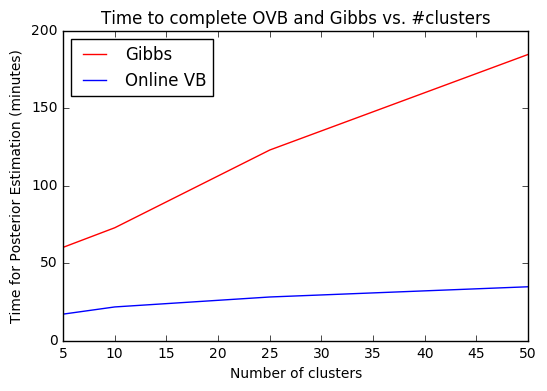
\includegraphics[width=0.5\textwidth]{figs/time}
    \caption{Comparison of the running times of each of the posterior estimation methods across various numbers of topics.}
    \label{fig:time}
\end{figure}

\begin{figure}
    \centering
    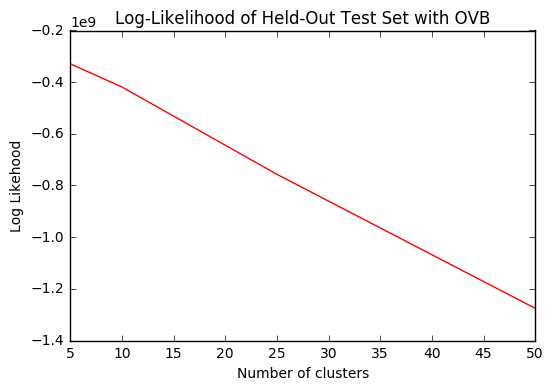
\includegraphics[width=0.5\textwidth]{figs/ll}
    \caption{Log-likelihood of the held-out testing set, across various numbers of topics.}
    \label{fig:ll}
\end{figure}

\begin{figure}
    \centering
    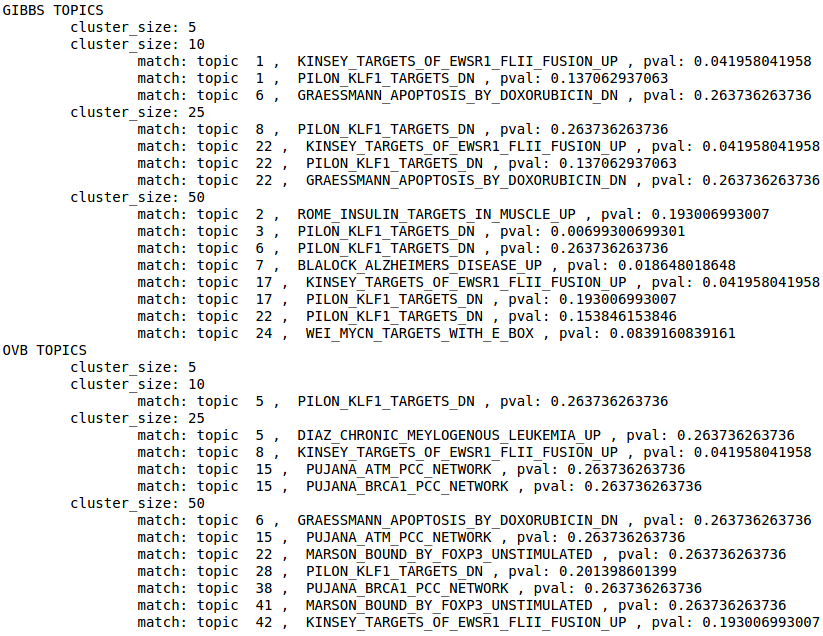
\includegraphics[width=1\textwidth]{figs/pathways}
    \caption{Matches between the gene collections found in LDA topics and published gene sets in \texttt{MSigDB}. Cluster size refers to the number of topics in the model}
    \label{fig:pathways}
\end{figure}

\begin{figure}
    \centering
    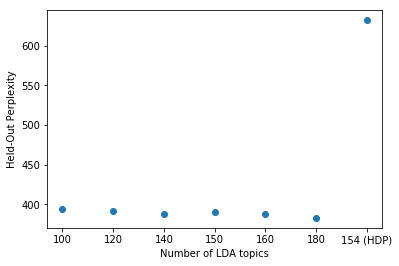
\includegraphics[width=0.5\textwidth]{figs/hdp-perplexity}
    \caption{Comparison of log-likelihood of the held-out testing set, under various LDA models and the HDP model.}
    \label{fig:hdp-perplexity}
\end{figure}

\begin{figure}
    \centering
    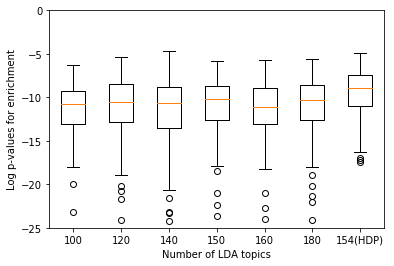
\includegraphics[width=0.5\textwidth]{figs/hdp-enrichment}
    \caption{Comparison of distributions of p-values from gene set enrichment analysis between LDA models and the HDP model.}
    \label{fig:hdp-enrichment}
\end{figure}

\begin{figure}
    \centering
    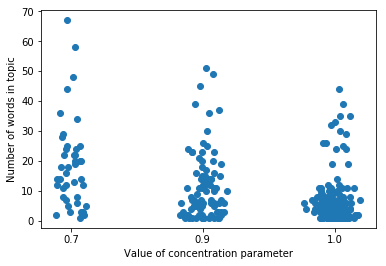
\includegraphics[width=0.5\textwidth]{figs/ibp_words_in_topic}
    \caption{Beeswarm plot of number of words per topic, for 3 different IBP-DP models with different concentration parameters. Each point represents one topic from its model}
    \label{fig:ibp_words_in_topic}
\end{figure}

\begin{figure}
    \centering
    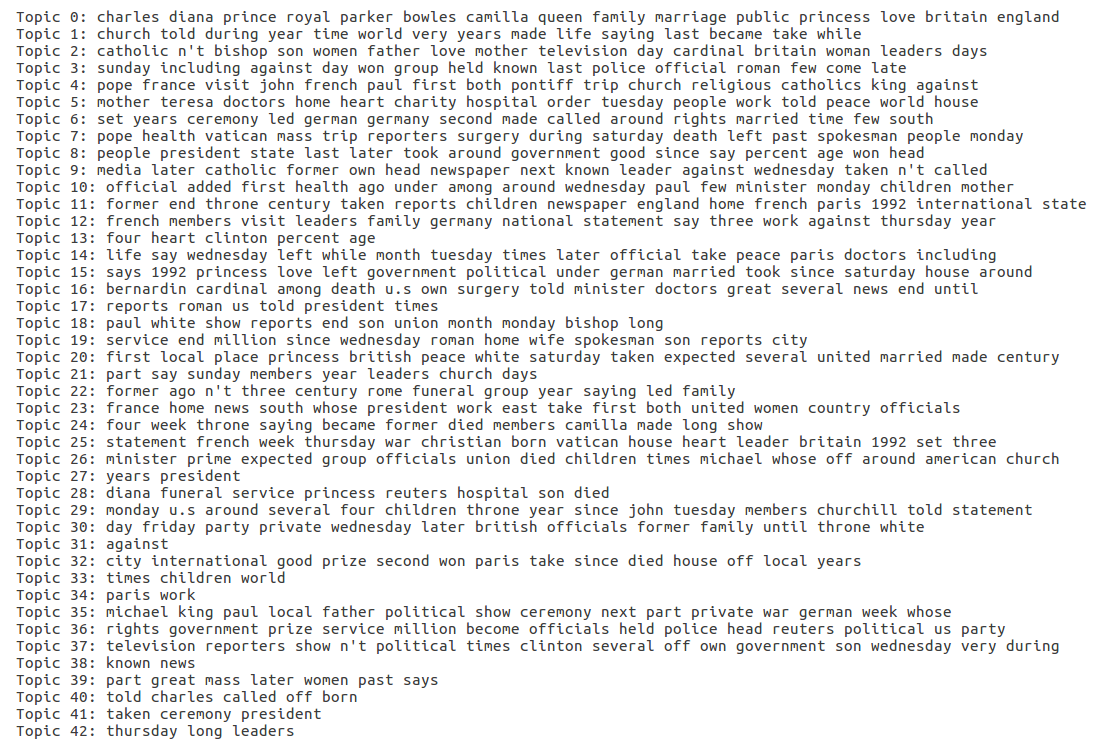
\includegraphics[width=1\textwidth]{figs/ibptopics}
    \caption{Topics from IBP-DP model trained on subset of Reuters dataset.}
    \label{fig:ibptopics}
\end{figure}

\begin{figure}
    \centering
    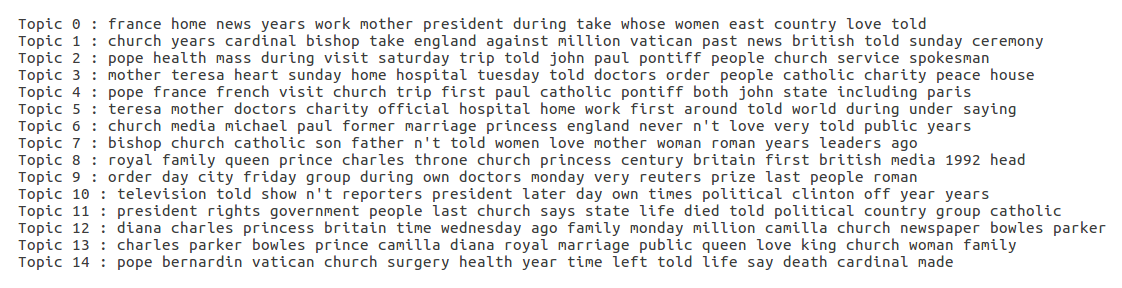
\includegraphics[width=1\textwidth]{figs/ldatopics}
    \caption{Topics from LDA model with 15 topics trained on subset of Reuters dataset.}
    \label{fig:ldatopics}
\end{figure}

\begin{figure}
    \centering
    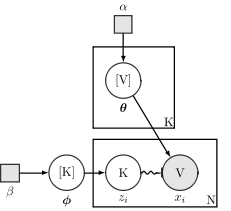
\includegraphics[width=0.3\textwidth]{figs/mixture}
    \caption{Finite \texttt{K}-sized mixture model currently implemented. $\theta$ is the parameter for every cluster component, represented from a categorical draw of over all genes. $z_i$ is the cluster assignment, and $\phi$ is the distribution of clusters. As usual, $\alpha, \beta$ are hyper-parameters.}
    \label{fig:plate}
\end{figure}

\end{document} 
